\documentclass[11pt,a4paper]{article}
\usepackage[margin=22mm]{geometry}
\usepackage[T1]{fontenc}
\usepackage{lmodern}
\usepackage{microtype}
\usepackage{amsmath,amssymb,mathtools,bm}
\usepackage{slashed}
\usepackage{booktabs,longtable,tabularx,array}
\usepackage{siunitx}
\usepackage{graphicx,subcaption,float}
\usepackage[dvipsnames]{xcolor}
\usepackage[colorlinks=true,allcolors=MidnightBlue]{hyperref}
\usepackage[nameinlink,noabbrev]{cleveref}
\usepackage{enumitem}
\usepackage{fancyhdr}
\usepackage{placeins}
\graphicspath{{../outputs/figures/}}
\sisetup{round-mode=places,round-precision=3,scientific-notation=true}
\allowdisplaybreaks
\setlist{nosep}
\pagestyle{fancy}
\setlength{\headheight}{14pt}
\fancyhf{}
\lhead{Mixed-current radiative QCD sum rules}
\rhead{\thepage}
\newcommand{\RegressionPass}{42/42}
\newcommand{\RegressionMaxRel}{9.13e-07}
\newcommand{\RegressionMaxAbs}{2.43e-06}
\newcommand{\NMonteCarlo}{1200}
\newcommand{\DsLowG}{-0.061}
\newcommand{\DsLowWidth}{0.482}
\newcommand{\DsHighG}{-0.017}
\newcommand{\DsHighWidth}{0.094}
\newcommand{\BsLowG}{-0.548}
\newcommand{\BsLowWidth}{1.589}
\newcommand{\BsHighG}{-0.484}
\newcommand{\BsHighWidth}{2.332}


\newcommand{\JA}{J_A}
\newcommand{\JB}{J_B}
\newcommand{\JL}{J_L}
\newcommand{\JH}{J_H}
\newcommand{\Mcal}{\mathcal M}
\newcommand{\PiT}{\Pi^{\mathrm T}}
\newcommand{\Twide}{\widehat T}
\newcommand{\GeV}{\mathrm{GeV}}
\newcommand{\keV}{\mathrm{keV}}
\newcommand{\tr}{\operatorname{Tr}}

\title{\textbf{Mixed-current external-photon QCD sum rules for}\\
$D_{s1},B_{s1}\to D_s^\ast,B_s^\ast\gamma$}
\author{Clean-room symbolic and numerical analysis}
\date{29 July 2026}

\begin{document}
\maketitle

\begin{abstract}
We construct a $2\times2$ QCD sum-rule matrix for the axial-vector and
derivative-tensor heavy-light currents, rotate it to lower and higher
$1^+$ channels, and combine the resulting residues with an
external-photon light-cone sum rule (LCSR).  The transition operator product
expansion (OPE) retains leading-order hard emission and Ball--Braun--Kivel
two- and three-particle photon distribution amplitudes (DAs) through twist
four.  Ordinary local vacuum-condensate transition terms are excluded; the
historical local heavy-line term is displayed only as a diagnostic.  The
tensor-current transition is derived at leading power, where
$\Twide_B=m_Q\Twide_A/(m_Q+m_s)$ after the double Borel transform.  Independent
Python and Wolfram Language implementations agree for \RegressionPass\
regression entries, with maximum material relative difference
\RegressionMaxRel.  From \NMonteCarlo\ accepted uncertainty samples per state
we obtain median radiative widths of \DsLowWidth, \DsHighWidth, \BsLowWidth,
and \BsHighWidth\ keV for $D_{s1}(2460)$, $D_{s1}(2536)$, a predicted lower
$B_{s1}^{L}$, and $B_{s1}(5830)$, respectively.  The distributions are broad
and non-Gaussian.  In particular, the transition Borel-mass variation is
large, so these results are exploratory rather than precision predictions.
\end{abstract}

\section{Scope and applicability}

The channels studied are
\begin{align}
D_{s1}(2460)^+&\to D_s^{\ast+}\gamma,&
D_{s1}(2536)^+&\to D_s^{\ast+}\gamma,\nonumber\\
B_{s1}^{L\,0}&\to B_s^{\ast0}\gamma,&
B_{s1}(5830)^0&\to B_s^{\ast0}\gamma .
\end{align}
They are heavy-light mesons with one strange spectator and an on-shell
photon.  An external-photon LCSR is therefore applicable.  The lower bottom
state is a model prediction, whereas $B_{s1}(5830)$ is established.  The
particle masses and experimental status are taken from the 2026 Particle
Data Group listings \cite{PDG2026}.  The photon DAs and their normalization
follow Ref.~\cite{BBK2003}; the pure-axial charm and bottom analyses used as
benchmarks are Refs.~\cite{Colangelo2005,Wang2008}.

This calculation has a sharply declared boundary.  It is leading order in
$\alpha_s$ and includes transition DAs through twist four.  The full
two-point AA, AB, and BB matrix is calculated.  For the transition only the
leading-power tensor projection is retained.  Subleading tensor kernels and
transition radiative corrections are not silently estimated as calculated
terms: correlated truncation uncertainties of 15\% in charm and 5\% in bottom
are assigned to the tensor projection, and both omissions remain explicit in
the validation ledger.

\section{Conventions, currents, and observable}

We use $g_{\mu\nu}=\operatorname{diag}(1,-1,-1,-1)$,
$\epsilon^{0123}=+1$, $\gamma_5=i\gamma^0\gamma^1\gamma^2\gamma^3$, and
$\sigma_{\mu\nu}=i[\gamma_\mu,\gamma_\nu]/2$.  The initial momentum is
$p'=p+q$, the photon satisfies $q^2=0$, and $e>0$.  The currents are
\begin{equation}
 \JA^\mu=\bar s\gamma^\mu\gamma_5Q,\qquad
 \JB^\mu={i\over m_Q+m_s}\bar s\sigma^{\mu\nu}p'_\nu\gamma_5Q,\qquad
 J_V^\mu=\bar s\gamma^\mu Q .
\end{equation}
The physical-current rotation is
\begin{equation}
\begin{pmatrix}\JL\\ \JH\end{pmatrix}
=R(\theta)\begin{pmatrix}\JA\\ \JB\end{pmatrix},\qquad
R(\theta)=
\begin{pmatrix}\sin\theta&\cos\theta\\
\cos\theta&-\sin\theta\end{pmatrix}.
\label{eq:rotation}
\end{equation}
The adopted angles are $\theta_D=38.4^\circ$ and
$\theta_B=35.264^\circ$, with angle scans included below.  The pole residues
are defined without hidden current-dependent factors,
\begin{equation}
\langle0|J_i^\mu|H_i(p',\eta)\rangle=f_i m_i\eta^\mu,\qquad
\langle0|J_V^\mu|V(p,\xi)\rangle=f_Vm_V\xi^\mu.
\end{equation}

For an on-shell $1^+\to1^-\gamma$ transition there are two independent
gauge-invariant multipoles.  We calculate the leading antisymmetric
structure
\begin{equation}
\mathcal A=ie\,g\,\epsilon_{\alpha\beta\rho\sigma}
\eta^\alpha\xi^{*\beta}\varepsilon^{*\rho}q^\sigma ,
\label{eq:amplitude}
\end{equation}
and set the second, higher-multipole form factor to zero at the retained
leading-power accuracy.  Replacing $\varepsilon$ by $q$ makes
\cref{eq:amplitude} vanish identically.  The corresponding width is
\begin{equation}
\Gamma(1^+\to1^-\gamma)=
{\alpha_{\rm em}g^2 k_\gamma^3(m_i^2+m_f^2)\over
3m_i^2m_f^2},\qquad
k_\gamma={m_i^2-m_f^2\over2m_i}.
\label{eq:width}
\end{equation}
Thus $g$ is dimensionless.

\section{Two-point matrix sum rule}

\subsection{Cut trace and exact-mass spectral densities}

Define
\begin{equation}
\Pi^{ij}_{\mu\nu}(p')=i\int d^4x\,e^{ip'\cdot x}
\langle0|T\{J^i_\mu(x)J^{j\dagger}_\nu(0)\}|0\rangle
=(-g_{\mu\nu}+p'_\mu p'_\nu/p'^2)\PiT_{ij}+\cdots .
\end{equation}
At leading order, the cut loop contains a heavy quark and an anti-strange
quark.  In the $p'$ rest frame, the transverse spin average is
\begin{equation}
{1\over3}\sum_{a=1}^3
\tr[(\slashed\ell-m_s)\Gamma_i^a(\slashed k+m_Q)
\bar\Gamma_j^a],
\quad
\Gamma_A^a=\gamma^a\gamma_5,\quad
\Gamma_B^a={i\sqrt{s}\over m_Q+m_s}\sigma^{a0}\gamma_5 .
\end{equation}
The two-body phase-space cut gives the exact-$m_s$ spectral matrix.  With
$S=m_Q+m_s$, $d=m_Q-m_s$, and
\begin{equation}
\lambda(s,m_Q^2,m_s^2)=[s-S^2][s-d^2],
\end{equation}
the entries are
\begin{align}
\rho_{AA}(s)&={\sqrt{\lambda}\over8\pi^2}
{(s-S^2)(d^2+2s)\over s^2},\label{eq:rhoaa}\\
\rho_{AB}(s)=\rho_{BA}(s)&={\sqrt{\lambda}\over8\pi^2}
{3d(s-S^2)\over Ss},\label{eq:rhoab}\\
\rho_{BB}(s)&={\sqrt{\lambda}\over8\pi^2}
{(s-S^2)(s+2d^2)\over S^2s}.\label{eq:rhobb}
\end{align}
All entries have dimension two and begin at the physical threshold $S^2$.
The symbolic determinant factorizes as
\begin{equation}
\det\rho(s)={\bigl(s-S^2\bigr)^3\bigl(s-d^2\bigr)^3
\over32\pi^4 S^2s^3}\ge0\qquad(s\ge S^2),
\label{eq:det}
\end{equation}
which checks spectral positivity as well as the AB normalization.

\subsection{Pre-Borel representation and local terms}

Before Borel transformation,
\begin{equation}
\PiT_{ij}(p'^2)=\int_{S^2}^{\infty}ds\,{\rho_{ij}(s)\over s-p'^2}
+\Pi^{(3)}_{ij}(p'^2)+\Pi^{(m_s)}_{ij}(p'^2)
+\Pi^{(5)}_{ij}(p'^2).
\end{equation}
The Borel rule used everywhere is
\begin{equation}
\mathcal B_{P^2\to M^2}{1\over(s-P^2)^n}
={e^{-s/M^2}\over(n-1)!(M^2)^{n-1}}.
\label{eq:borel}
\end{equation}
Writing $\langle\bar ss\rangle=s_s$ and
$\langle\bar s g_s\sigma Gs\rangle=m_0^2s_s$, the local Borel matrices are
\begin{align}
\Twide\Pi^{(3)}
&=s_s e^{-m_Q^2/M^2}
\begin{pmatrix}
m_Q&m_Q^2/S\\m_Q^2/S&m_Q^3/S^2
\end{pmatrix},\label{eq:d3}\\
\Twide\Pi^{(m_s)}
&=s_s e^{-m_Q^2/M^2}
\left(-{m_Q^2m_s\over2M^2}
+{m_Q^3m_s^2\over2M^4}\right)
\begin{pmatrix}1&m_Q/S\\m_Q/S&m_Q^2/S^2\end{pmatrix},
\label{eq:d3ms}\\
\Twide\Pi^{(5)}&=e^{-m_Q^2/M^2}
\begin{pmatrix}
-{m_0^2s_s m_Q^3\over4M^4}&
-{m_0^2s_s\over4S}\left({m_Q^4\over M^4}-{m_Q^2\over M^2}-1\right)\\
\text{sym.}&
{m_0^2s_s\over S^2}\left(-{m_Q^5\over4M^4}
+{m_Q^3\over2M^2}\right)
\end{pmatrix}.
\label{eq:d5}
\end{align}
The continuum-subtracted basis matrix is therefore
\begin{equation}
\Twide\Pi_{ij}(M^2,s_0)=
\int_{S^2}^{s_0}ds\,e^{-s/M^2}\rho_{ij}(s)
+\Twide\Pi^{(3)}_{ij}+\Twide\Pi^{(m_s)}_{ij}
+\Twide\Pi^{(5)}_{ij}.
\label{eq:pi2pt}
\end{equation}
No off-diagonal element is set to zero.  The physical matrix is
\begin{equation}
\Twide\Pi^{\rm phys}=R(\theta)\Twide\Pi R^T(\theta).
\end{equation}
For state $a=L,H$,
\begin{equation}
f_a(M^2,s_0)={e^{m_a^2/(2M^2)}\over m_a}
\sqrt{\Twide\Pi^{\rm phys}_{aa}},\qquad
m_{\rm SR}^2={-\partial_{(1/M^2)}\Twide\Pi^{\rm phys}_{aa}
\over\Twide\Pi^{\rm phys}_{aa}}.
\label{eq:residue}
\end{equation}
The remaining rotated off-diagonal correlation is reported as a diagnostic,
not erased by hand.

For the vector final state, the perturbative density is
\begin{equation}
\rho_V(s)={\sqrt{\lambda}\over8\pi^2}
\left[2-{m_Q^2+m_s^2-6m_Qm_s\over s}
-{(m_Q^2-m_s^2)^2\over s^2}\right],
\end{equation}
and the local AA coefficients in
\cref{eq:d3,eq:d3ms,eq:d5} change sign.  Its residue is extracted with the
analogue of \cref{eq:residue}.

\subsection{Window criteria}

The pole contribution is the continuum-subtracted correlator divided by the
same OPE with the perturbative upper limit extended to infinity.  Accepted
two-point points obey
\begin{equation}
\mathrm{PC}\ge0.40,\qquad
{|\Pi^{(5)}|\over|\Pi|}\le0.10,\qquad
\left|{m_{\rm SR}\over m_{\rm phys}}-1\right|\le0.05.
\end{equation}
The resulting windows and diagnostics are:
\begin{table}[H]
\centering\small
\begin{tabular}{lcccccc}
\toprule
State & $M^2$ [GeV$^2$] & $s_0$ [GeV$^2$] & accepted & PC & $|d=5|/|\Pi|$ & $m_{\rm SR}$ [GeV]\\
\midrule
$D_{s1}(2460)$ & 2.0--3.0 & 7.50--8.50 & 29/30 & 0.41--0.71 & 0.023 & 2.418--2.506 \\
$D_{s1}(2536)$ & 2.0--3.0 & 8.50--10.00 & 18/30 & 0.41--0.67 & 0.097 & 2.428--2.655 \\
$B_{s1}^{L}$ & 8.0--11.0 & 40.00--42.00 & 30/30 & 0.42--0.66 & 0.002 & 5.649--5.785 \\
$B_{s1}(5830)$ & 7.0--9.0 & 42.00--44.00 & 30/30 & 0.40--0.64 & 0.037 & 5.730--5.896 \\
\bottomrule
\end{tabular}

\caption{Accepted two-point windows.  The predicted lower bottom mass used
for the residue extraction is \SI{5.75}{GeV}.}
\label{tab:windows}
\end{table}

\section{External-photon transition sum rule}

\subsection{Correlation function, contraction, and OPE routing}

For basis current $i=A,B$,
\begin{equation}
T^i_{\mu\nu}(p,q)=i\int d^4x\,e^{ip\cdot x}
\langle\gamma(q,\varepsilon)|T\{J^\dagger_{V\mu}(x)J^i_\nu(0)\}|0\rangle .
\end{equation}
The Wick contraction is fixed as
\begin{equation}
T^i_{\mu\nu}=-i\int d^4x\,e^{ip\cdot x}
\langle\gamma|\bar s(x)\gamma_\mu S_Q(x,0)
\Gamma^i_\nu s(0)|0\rangle,
\end{equation}
which fixes the global fermion sign.  The light-cone propagators used to
generate the nonlocal terms include
\begin{align}
S_s^{(0)}(x)&={i\slashed x\over2\pi^2x^4}
-{m_s\over4\pi^2x^2},\\
S_Q^{(\gamma)}(x,0)&=-ie_Q\int d^4y\,
S_Q^{(0)}(x-y)\slashed A(y)S_Q^{(0)}(y),\\
S_Q^{(G)}(k)&=-{ig_s\over4}{G_{\alpha\beta}\bigl[
\sigma^{\alpha\beta}(\slashed k+m_Q)
+(\slashed k+m_Q)\sigma^{\alpha\beta}\bigr]\over(k^2-m_Q^2)^2}.
\end{align}
For the nonlocal strange propagator we retain the free part and the
one-gluon light-cone insertion.  Ordinary vacuum-condensate pieces are not
inserted into the transition correlator.  This prevents a local
$\langle\bar ss\rangle$ term from being mixed with the external-photon DA
sum rule.

The needed two-particle photon matrix elements are, schematically,
\begin{align}
\langle\gamma|\bar s(x)\sigma_{\alpha\beta}s(0)|0\rangle
&=-ie_s s_s(\varepsilon_\alpha q_\beta-\varepsilon_\beta q_\alpha)
\int_0^1du\,e^{iuq\cdot x}
\left[\chi\phi_\gamma(u)+{x^2\over16}{\cal A}(u)\right]+\cdots,\\
\langle\gamma|\bar s(x)\gamma_\alpha s(0)|0\rangle
&=e_s f_{3\gamma}\left(\varepsilon_\alpha
-q_\alpha{\varepsilon\cdot x\over q\cdot x}\right)
\int_0^1du\,e^{iuq\cdot x}\psi^v(u),\\
\langle\gamma|\bar s(x)\gamma_\alpha\gamma_5s(0)|0\rangle
&=-{e_s f_{3\gamma}\over4}\epsilon_{\alpha\beta\rho\sigma}
\varepsilon^\beta q^\rho x^\sigma
\int_0^1du\,e^{iuq\cdot x}\psi^a(u).
\end{align}
The three-particle set
$\{{\cal S},\widetilde{\cal S},{\cal A},{\cal V},
{\cal T}_{1,2,3,4}\}$ follows Ref.~\cite{BBK2003}.  Their explicit conformal
forms and the combinations entering this projection are listed in
\cref{app:das}.

\subsection{Pre-Borel kernels}

Let
\begin{equation}
D(u)=m_Q^2-(1-u)p^2-u p'^2,\quad
u_0={M_1^2\over M_1^2+M_2^2},\quad
\Mcal^2={M_1^2M_2^2\over M_1^2+M_2^2}.
\end{equation}
The double-Borel identity is
\begin{equation}
\mathcal B_{M_1^2}\mathcal B_{M_2^2}{1\over D(u)^n}
={(\Mcal^2)^{2-n}\over\Gamma(n)}
e^{-m_Q^2/\Mcal^2}\delta(u-u_0).
\label{eq:doubleborel}
\end{equation}
We take $M_1^2=M_2^2=2M^2$, so $u_0=1/2$ and $\Mcal^2=M^2$.
Up to the common Lorentz structure, the pre-Borel ledger is
\begin{align}
T_{\rm hard}&=\int_{S^2}^{\infty}ds\,
{\rho_T(s)\over(s-p^2)(s-p'^2)},\label{eq:prehard}\\
T_{\rm tw2}&=e_s m_Qs_s\chi\int_0^1du\,{\phi_\gamma(u)\over D(u)},\\
T_{\rm tw4,2p}&=e_s m_Qs_s\int_0^1du\left[
-{m_Q^2{\cal A}(u)\over2D(u)^3}
-{(1-u)H_\gamma(u)+\bar H_\gamma(u)\over D(u)^2}
+{4m_Q^2\bar H_\gamma(u)\over D(u)^3}\right],\\
T_{\rm tw3,2p}&=e_s f_{3\gamma}\int_0^1du\left[
{C_1(u)\over D(u)}-{2m_Q^2\Psi^v(u)\over D(u)^2}\right],
\end{align}
where
\begin{equation}
C_1(u)={(1-u)\psi^{a\,\prime}(u)\over4}
-{\psi^a(u)\over4}-\Psi^v(u)+(1-u)\psi^v(u),
\end{equation}
$H_\gamma(u)=\int_0^u h_\gamma(v)dv$,
$\bar H_\gamma(u)=\int_0^u(u-v)h_\gamma(v)dv$, and
$\Psi^v(u)=\int_0^u\psi^v(v)dv$.  The three-particle twist-four kernel is
proportional to $D^{-2}{\cal F}_2$, and the twist-three kernel to
$D^{-1}{\cal F}_3$, with their exact integration domains in
\cref{app:das}.

The hard spectral density, including both quark charges and exact $m_s$, is
\begin{align}
\rho_T(s)&={3m_sm_Q\over4\pi^2}
\left[e_s\ln{a_s-\sqrt\lambda\over a_s+\sqrt\lambda}
+e_Q\ln{a_Q-\sqrt\lambda\over a_Q+\sqrt\lambda}\right],\\
a_s&=s-m_Q^2+m_s^2,\qquad a_Q=s-m_s^2+m_Q^2 .
\end{align}
Changing $c$ to $b$ therefore changes both $m_Q$ and $e_Q$.

\subsection{Post-Borel ledger and physical projection}

Define $E=e^{-m_Q^2/M^2}$, $E_0=e^{-s_0/M^2}$, and evaluate all DAs at
$u_0$.  The continuum-subtracted terms are
\begin{align}
\Twide T_{\rm hard}&=\int_{S^2}^{s_0}ds\,e^{-s/M^2}\rho_T(s),\\
\Twide T_{\rm tw2}&=e_sm_Qs_s\chi M^2(E-E_0)\phi_\gamma,\\
\Twide T_{\rm tw4,2p}&=e_sm_Qs_sE\left[
-{m_Q^2\over4M^2}{\cal A}
-(1-u_0)H_\gamma-\bar H_\gamma
\left({2m_Q^2\over M^2}\right)\bar H_\gamma\right],\\
\Twide T_{\rm tw3,2p}&=e_sf_{3\gamma}M^2(E-E_0)
\left[{(1-u_0)\psi^{a\,\prime}\over4}-{\psi^a\over4}
-(1+2m_Q^2/M^2)\Psi^v+(1-u_0)\psi^v\right],\\
\Twide T_{\rm tw4,3p}&=m_Qe_ss_sE\,I_{{\cal F}_2},\\
\Twide T_{\rm tw3,3p}&=-e_sf_{3\gamma}M^2(E-E_0)I_{{\cal F}_3}.
\label{eq:postterms}
\end{align}
The quoted axial-basis invariant is the sum of precisely these six entries.
For comparison only, the historical local term
\begin{equation}
\Twide T_{\rm local,diag}=e_Qm_Qs_sE
\left[1-{m_s^2\over M^2}\left(1-{m_Q^2\over M^2}\right)\right]
\end{equation}
is printed in every term ledger, but it is excluded from all quoted
couplings.

For the tensor current the twist-two trace ratio before Borel transformation
is
\begin{equation}
{T_B^{(2)}\over T_A^{(2)}}={k^2\over m_Q(m_Q+m_s)}.
\end{equation}
Using $k^2/(m_Q^2-k^2)=m_Q^2/(m_Q^2-k^2)-1$, the contact term has zero Borel
image and the retained leading-power relation becomes
\begin{equation}
\Twide T_B={m_Q\over m_Q+m_s}\Twide T_A.
\label{eq:tensorprojection}
\end{equation}
We apply \cref{eq:tensorprojection} term by term through twist four.  This is
the stated leading-power truncation, not a claim that all subleading
tensor-current kernels have been calculated.

Let $r_{aA}$ and $r_{aB}$ be row $a$ of $R(\theta)$.  The physical invariant
and coupling are
\begin{align}
\Twide T_a&=r_{aA}\Twide T_A+r_{aB}\Twide T_B,\\
g_a(M^2,s_0)&={e^{(m_a^2+m_V^2)/(2M^2)}
\over f_af_Vm_am_V}\Twide T_a .
\label{eq:coupling}
\end{align}
The separate A and B components are retained in the output to expose
constructive or destructive interference.

\section{Inputs and uncertainty protocol}

The fixed-scale LO inputs are $m_c=\SI{1.27(2)}{GeV}$,
$m_b=\SI{4.18(3)}{GeV}$, $m_s=\SI{0.093(11)}{GeV}$,
$\langle\bar qq\rangle=-(0.24\pm0.01)^3\GeV^3$,
$\langle\bar ss\rangle/\langle\bar qq\rangle=0.8\pm0.1$,
$m_0^2=0.8\pm0.1\GeV^2$, $\chi=-3.15\pm0.30\GeV^{-2}$, and
$f_{3\gamma}=-(3.9\pm2.0)\times10^{-3}\GeV^2$ at $\mu=1$ GeV.  The DA shape
parameters are $\omega_\gamma^V=3.8\pm1.8$,
$\omega_\gamma^A=-2.1\pm1.0$, $\kappa=0.2\pm0.2$,
$\zeta_1=0.4\pm0.2$, and $\zeta_2=0.3\pm0.2$.  The complete source,
unit, scale, status, and note for every input appears in
\path{inputs/input_provenance.csv}.

We use \NMonteCarlo\ reproducible samples per state (seed 20260729).  External
inputs, condensates, DA parameters, mixing angles, Borel variables, and
thresholds are varied simultaneously.  Accepted two-point points must satisfy
the gates above.  The tensor truncation nuisance is correlated across
transition terms within a sample.  The reported central value is the median
and the interval is the 16th--84th percentile range.  Because $g$ may cross
zero, the width distribution is strongly non-Gaussian; consequently a width
constructed by squaring the median $g$ need not equal the median width.

\section{Results}

\subsection{Residues, couplings, and widths}

\begin{table}[H]
\centering\small
\resizebox{\textwidth}{!}{\begin{tabular}{lcccc}
\toprule
State & $g$ & $\Gamma_\gamma$ [keV] & $f_i$ [GeV] & $f_V$ [GeV]\\
\midrule
$D_{s1}(2460)$ & $-0.061_{-0.160}^{+0.174}$ & $0.482_{-0.434}^{+1.609}$ & $0.404_{-0.018}^{+0.020}$ & $0.253_{-0.010}^{+0.008}$ \\
$D_{s1}(2536)$ & $-0.017_{-0.069}^{+0.058}$ & $0.094_{-0.089}^{+0.520}$ & $0.166_{-0.012}^{+0.014}$ & $0.253_{-0.010}^{+0.008}$ \\
$B_{s1}^{L}$ & $-0.548_{-0.339}^{+0.320}$ & $1.589_{-1.298}^{+2.703}$ & $0.501_{-0.017}^{+0.018}$ & $0.300_{-0.009}^{+0.009}$ \\
$B_{s1}(5830)$ & $-0.484_{-0.425}^{+0.286}$ & $2.332_{-1.925}^{+5.735}$ & $0.098_{-0.008}^{+0.014}$ & $0.300_{-0.009}^{+0.009}$ \\
\bottomrule
\end{tabular}
}
\caption{Monte Carlo medians and 16th--84th percentile intervals.  The sign
of $g$ follows \cref{eq:amplitude}; the width is sign independent.}
\label{tab:results}
\end{table}

For $D_{s1}(2460)$ the interval in $g$ crosses zero; its width distribution
therefore has a long upper tail.  The higher charm state has a destructive A/B
interference and an even smaller median coupling.  The bottom medians are
larger in magnitude, but the transition Borel dependence is also more severe.
Using the measured total widths where available gives:
\begin{table}[H]
\centering\small
\begin{tabular}{lcc}
\toprule
State & central radiative branching fraction & experimental status\\
\midrule
$D_{s1}(2536)$ & \num{1.019e-04} & possibly seen; no branching fraction \\
$B_{s1}(5830)$ & \num{4.664e-03} & mode not observed \\
\bottomrule
\end{tabular}

\caption{Derived central branching fractions.  The $B_{s1}(5830)$ entry uses
the PDG central total width and is therefore especially uncertain.}
\end{table}

The central OPE ledger, in $\GeV^4$, is shown in \cref{tab:terms}.  The last
column is excluded from the quoted total.
\begin{table}[H]
\centering\scriptsize
\resizebox{\textwidth}{!}{\begin{tabular}{lrrrrrrr}
\toprule
State & hard & tw2 & tw3(2p) & tw3(3p) & tw4(2p) & tw4(3p) & local diag.\\
\midrule
$D_{s1}(2460)$ & \num{0.019} & \num{-0.051} & \num{0.013} & \num{0.013} & \num{-8.631e-04} & \num{-6.133e-21} & \num{-0.007} \\
$D_{s1}(2536)$ & \num{0.020} & \num{-0.054} & \num{0.014} & \num{0.014} & \num{-8.631e-04} & \num{-6.133e-21} & \num{-0.007} \\
$B_{s1}^{L}$ & \num{0.013} & \num{-0.023} & \num{0.002} & \num{0.002} & \num{-0.004} & \num{-1.515e-21} & \num{8.400e-04} \\
$B_{s1}(5830)$ & \num{0.013} & \num{-0.023} & \num{0.002} & \num{0.002} & \num{-0.004} & \num{-1.515e-21} & \num{8.400e-04} \\
\bottomrule
\end{tabular}
}
\caption{Transition term decomposition at the central $(M^2,s_0)$ point.
``2p'' and ``3p'' denote two- and three-particle photon DAs.}
\label{tab:terms}
\end{table}

\subsection{Stability}

The relative full-range variations are:
\begin{table}[H]
\centering\small
\begin{tabular}{lrrrr}
\toprule
State & $\Delta_{M^2}g$ & $\Delta_{s_0}g$ & $\Delta_{M^2}\Gamma$ & $\Delta_{s_0}\Gamma$\\
\midrule
$D_{s1}(2460)$ & 39.8\% & 3.4\% & 87.1\% & 6.7\% \\
$D_{s1}(2536)$ & 40.7\% & 3.3\% & 89.3\% & 6.6\% \\
$B_{s1}^{L}$ & 108.6\% & 1.2\% & 279.9\% & 2.3\% \\
$B_{s1}(5830)$ & 113.4\% & 0.9\% & 295.7\% & 1.9\% \\
\bottomrule
\end{tabular}

\caption{Relative scan variation $(\max-\min)/|\mathrm{mean}|$.}
\label{tab:stability}
\end{table}
Threshold sensitivity is small on the declared grids, but the Borel-mass
sensitivity is not.  The coupling changes by about 40\% in charm and more
than 100\% in bottom, while the width variation is larger still.  The
uncertainty intervals in \cref{tab:results} reflect this behavior.  No
plateau claim is made for the bottom transition.

\begin{figure}[p]
\centering
\begin{subfigure}{0.49\textwidth}
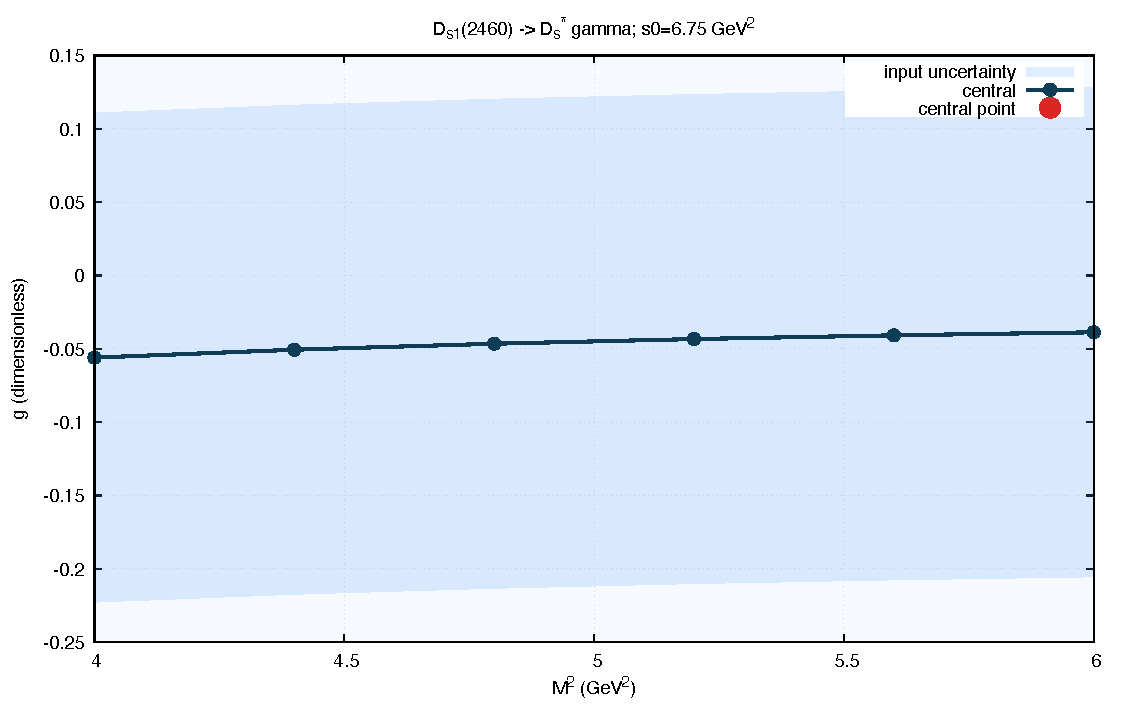
\includegraphics[width=\linewidth]{Ds1_2460_coupling_vs_M2.pdf}
\caption{$D_{s1}(2460)$: $g$ vs.\ $M^2$.}
\end{subfigure}
\begin{subfigure}{0.49\textwidth}
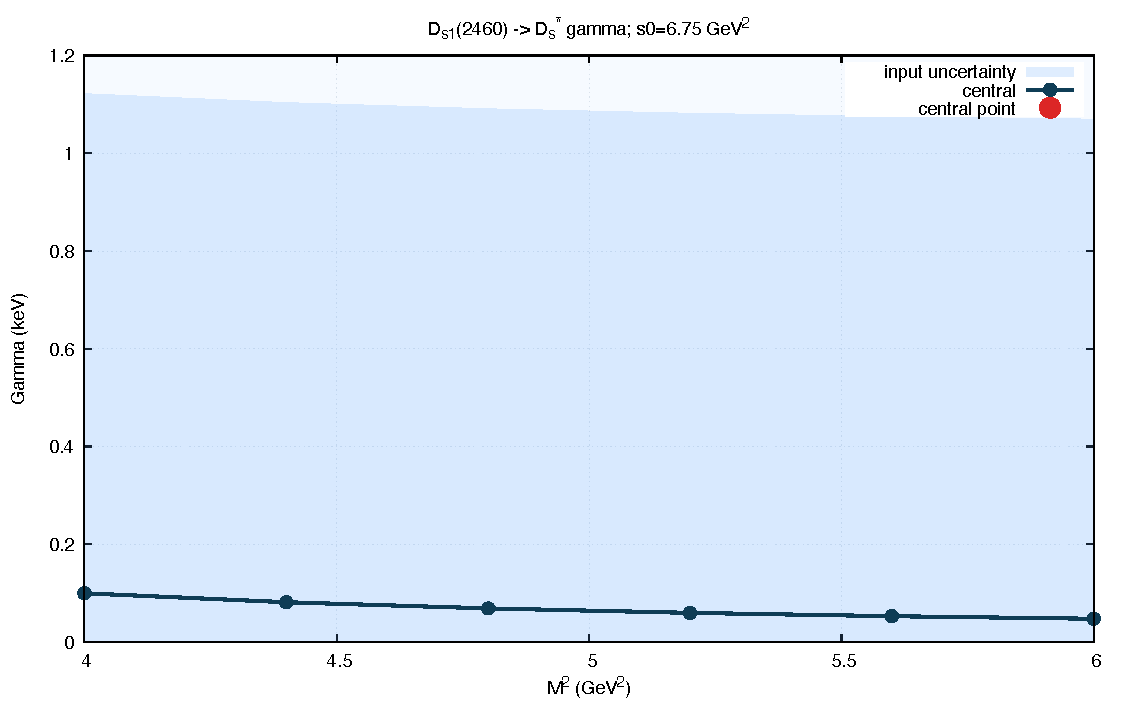
\includegraphics[width=\linewidth]{Ds1_2460_width_vs_M2.pdf}
\caption{$D_{s1}(2460)$: width vs.\ $M^2$.}
\end{subfigure}
\begin{subfigure}{0.49\textwidth}
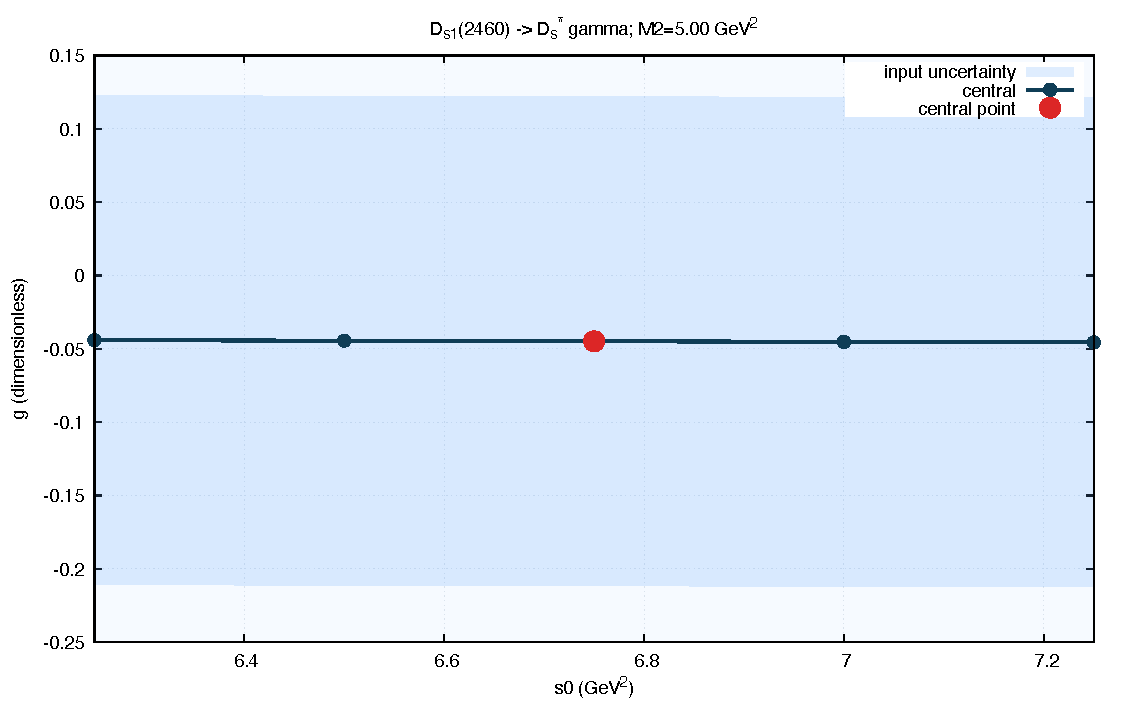
\includegraphics[width=\linewidth]{Ds1_2460_coupling_vs_s0.pdf}
\caption{$D_{s1}(2460)$: $g$ vs.\ $s_0$.}
\end{subfigure}
\begin{subfigure}{0.49\textwidth}
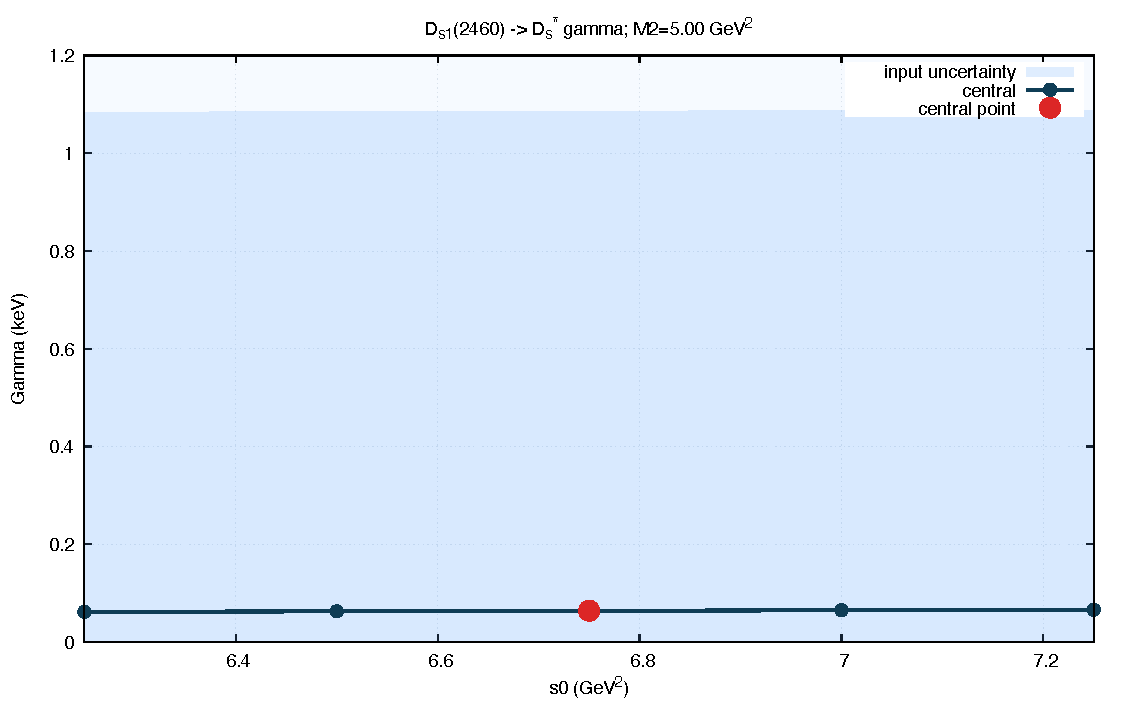
\includegraphics[width=\linewidth]{Ds1_2460_width_vs_s0.pdf}
\caption{$D_{s1}(2460)$: width vs.\ $s_0$.}
\end{subfigure}
\caption{The four principal stability scans for the lower charm state.}
\label{fig:dsstability}
\end{figure}

\begin{figure}[p]
\centering
\begin{subfigure}{0.49\textwidth}
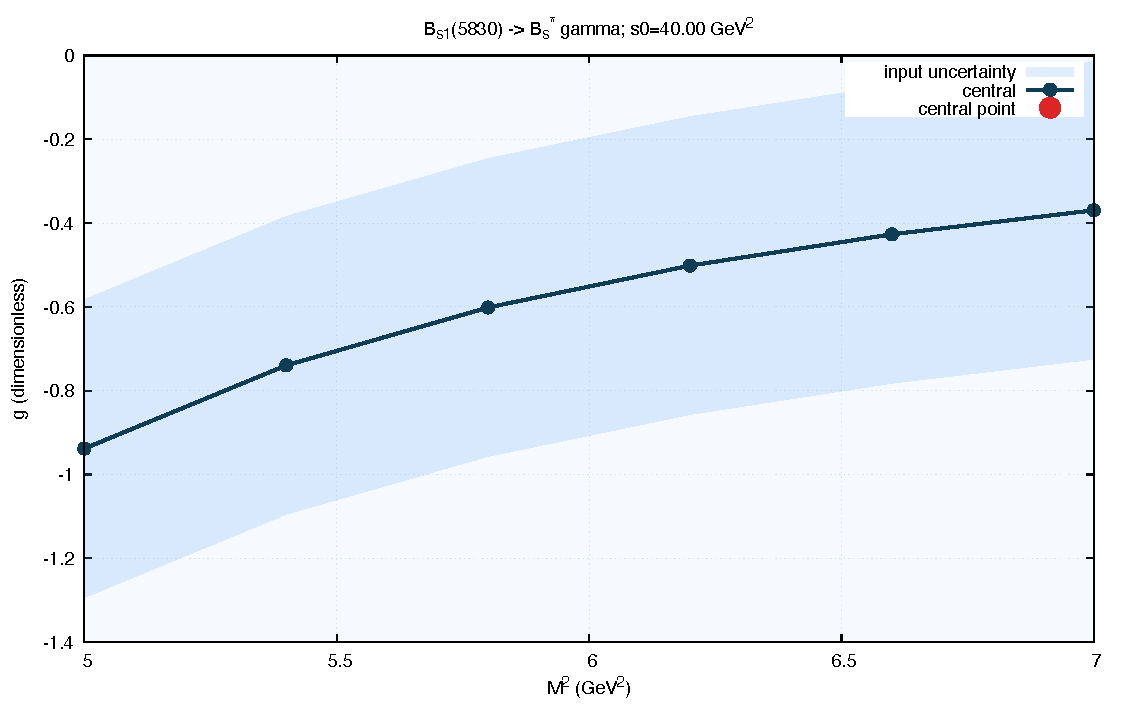
\includegraphics[width=\linewidth]{Bs1_5830_coupling_vs_M2.pdf}
\caption{$B_{s1}(5830)$: $g$ vs.\ $M^2$.}
\end{subfigure}
\begin{subfigure}{0.49\textwidth}
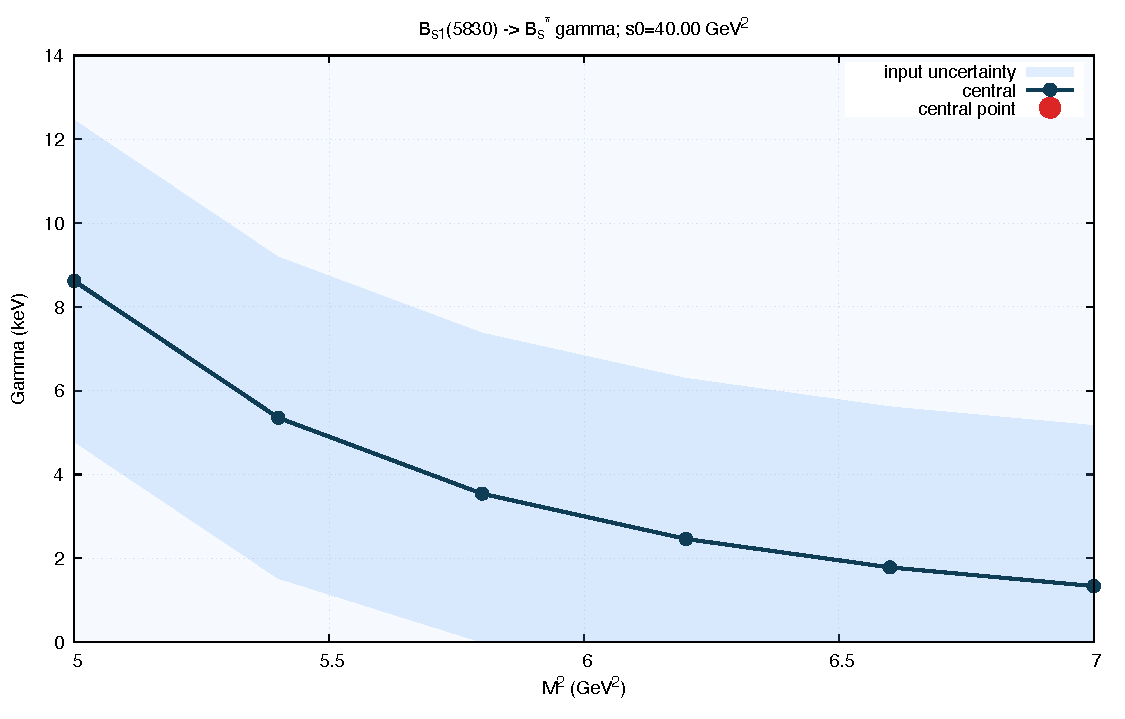
\includegraphics[width=\linewidth]{Bs1_5830_width_vs_M2.pdf}
\caption{$B_{s1}(5830)$: width vs.\ $M^2$.}
\end{subfigure}
\begin{subfigure}{0.49\textwidth}
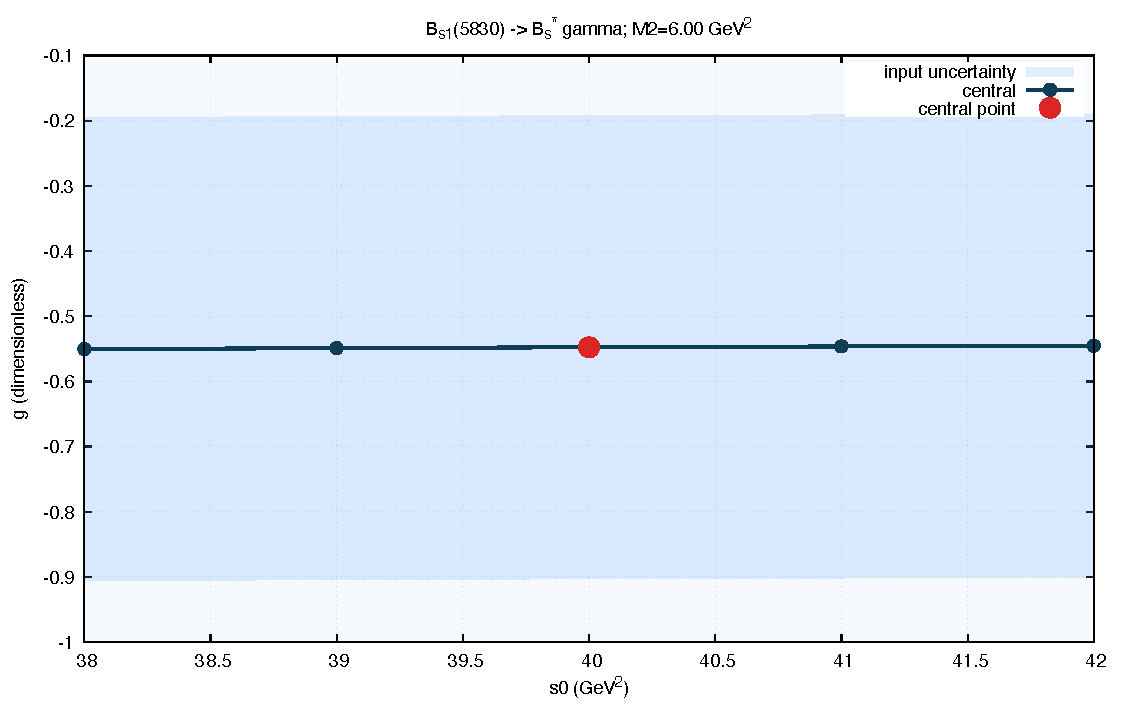
\includegraphics[width=\linewidth]{Bs1_5830_coupling_vs_s0.pdf}
\caption{$B_{s1}(5830)$: $g$ vs.\ $s_0$.}
\end{subfigure}
\begin{subfigure}{0.49\textwidth}
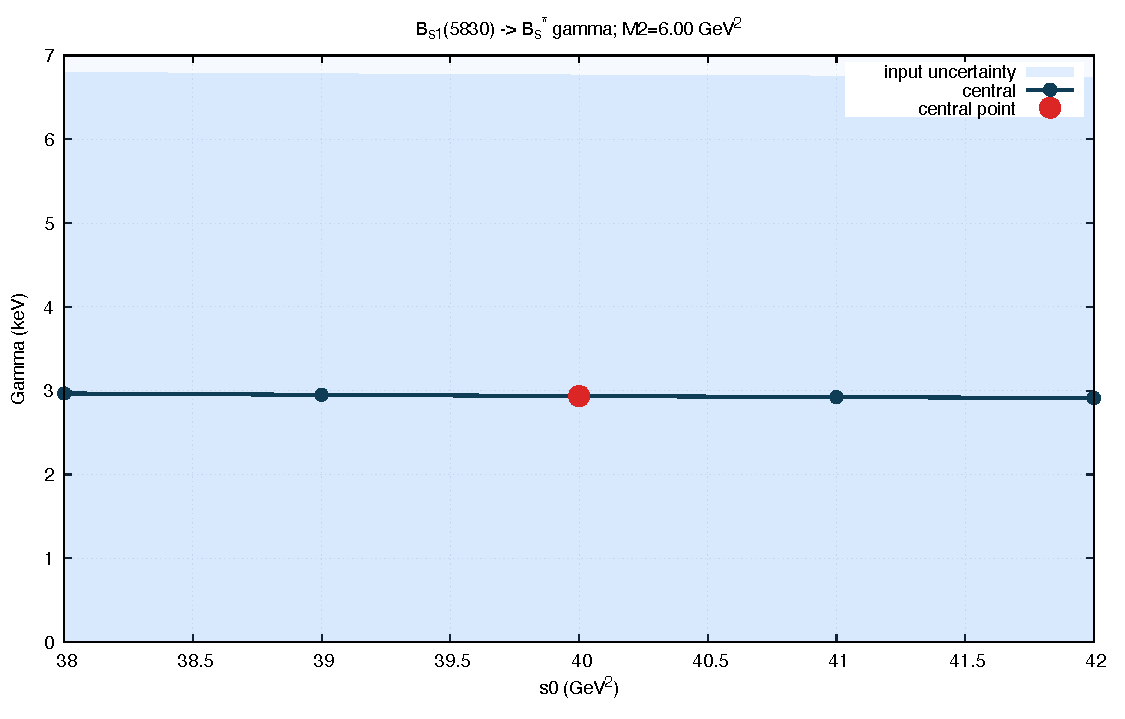
\includegraphics[width=\linewidth]{Bs1_5830_width_vs_s0.pdf}
\caption{$B_{s1}(5830)$: width vs.\ $s_0$.}
\end{subfigure}
\caption{The four principal stability scans for the higher bottom state.}
\label{fig:bsstability}
\end{figure}
\FloatBarrier

\begin{figure}[H]
\centering
\begin{subfigure}{0.49\textwidth}
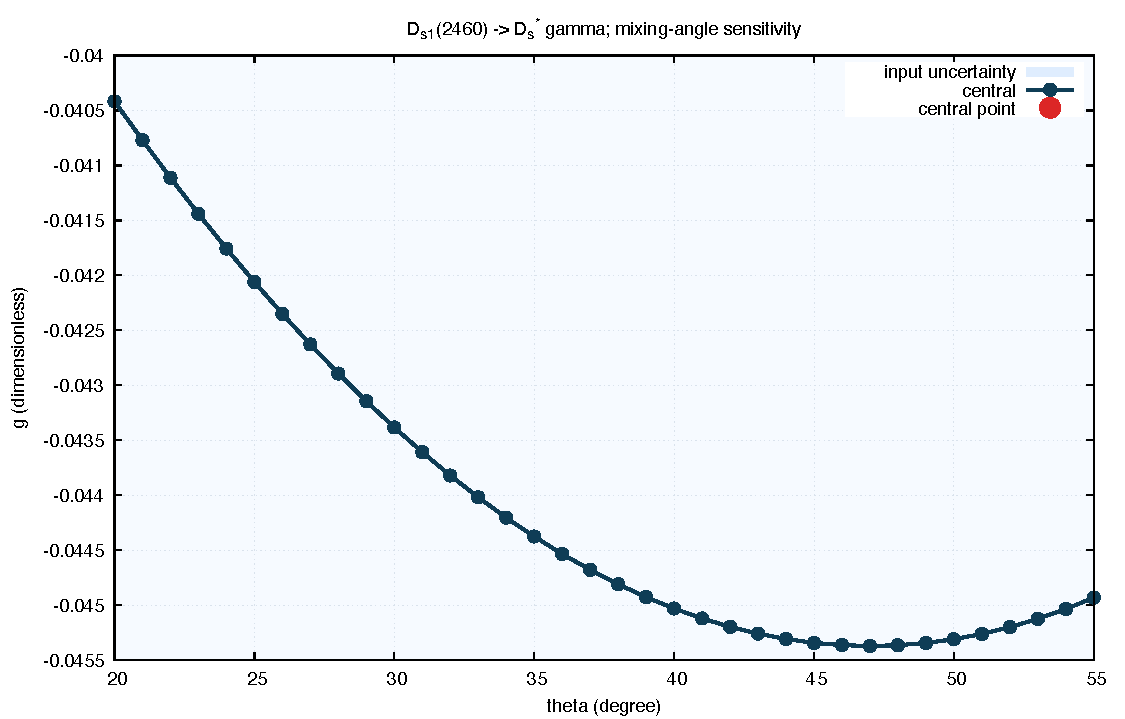
\includegraphics[width=\linewidth]{Ds1_2460_coupling_vs_angle.pdf}
\caption{Charm lower-state angle scan.}
\end{subfigure}
\begin{subfigure}{0.49\textwidth}
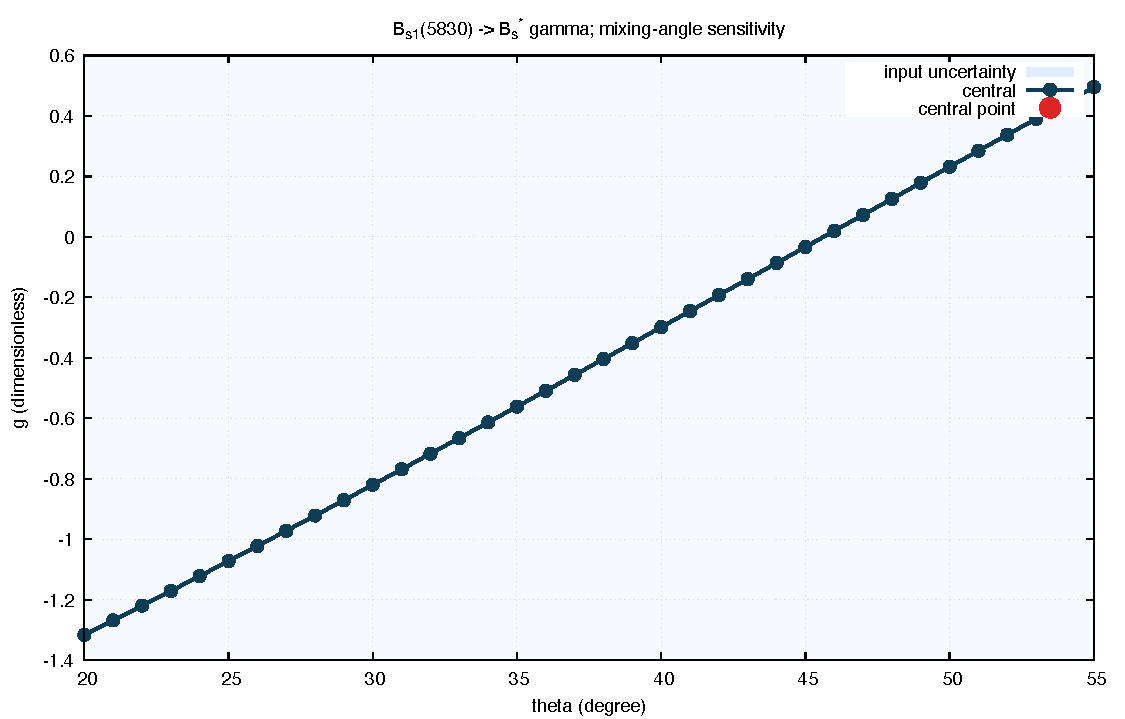
\includegraphics[width=\linewidth]{Bs1_5830_coupling_vs_angle.pdf}
\caption{Bottom higher-state angle scan.}
\end{subfigure}
\caption{Mixing-angle sensitivity.  Zero crossings expose destructive
interference between the A and B current components.}
\end{figure}

\begin{figure}[H]
\centering
\begin{subfigure}{0.32\textwidth}
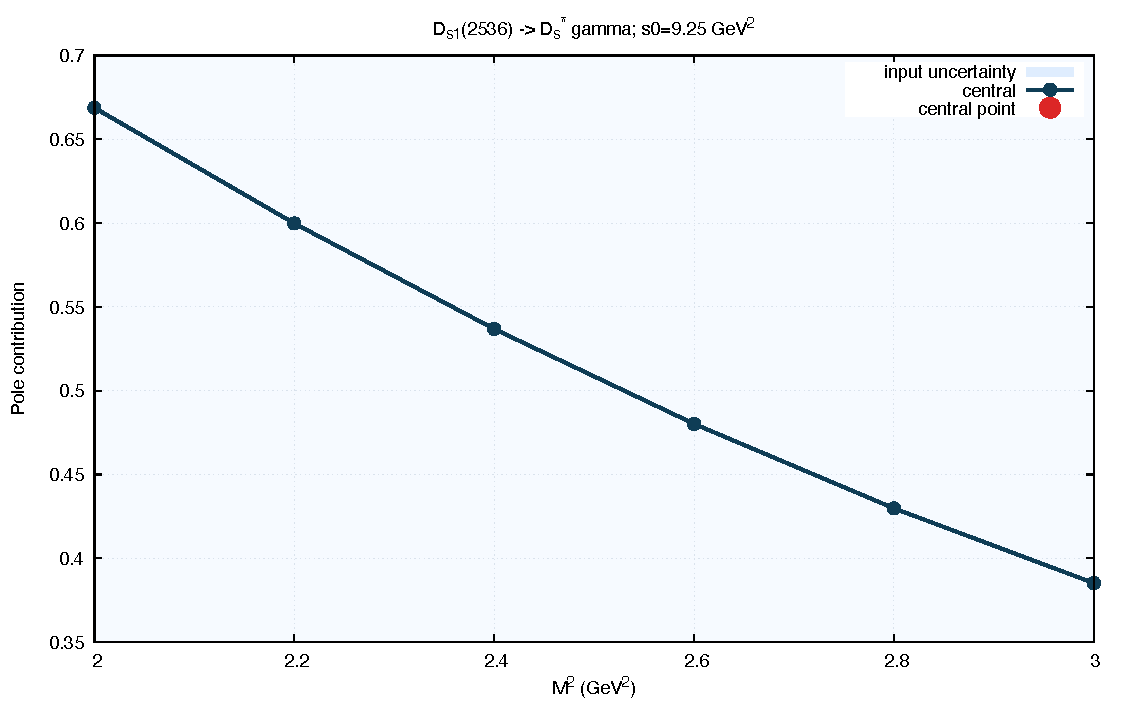
\includegraphics[width=\linewidth]{Ds1_2536_pc_vs_M2.pdf}
\caption{pole contribution}
\end{subfigure}
\begin{subfigure}{0.32\textwidth}
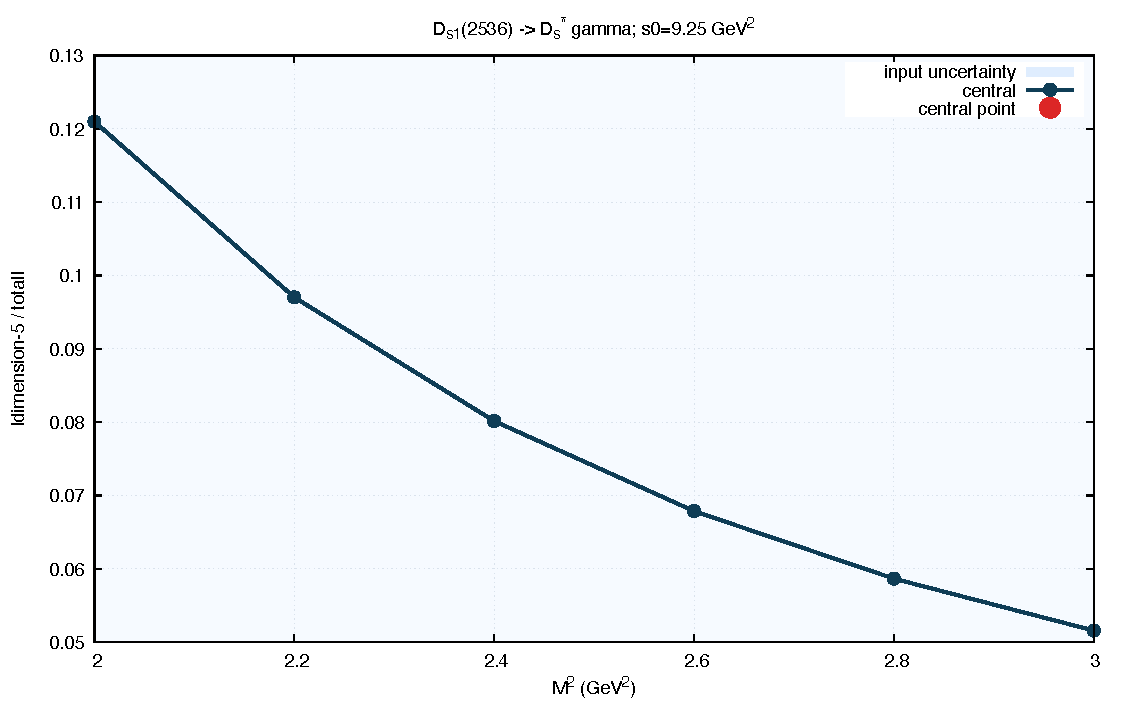
\includegraphics[width=\linewidth]{Ds1_2536_d5frac_vs_M2.pdf}
\caption{dimension-five fraction}
\end{subfigure}
\begin{subfigure}{0.32\textwidth}
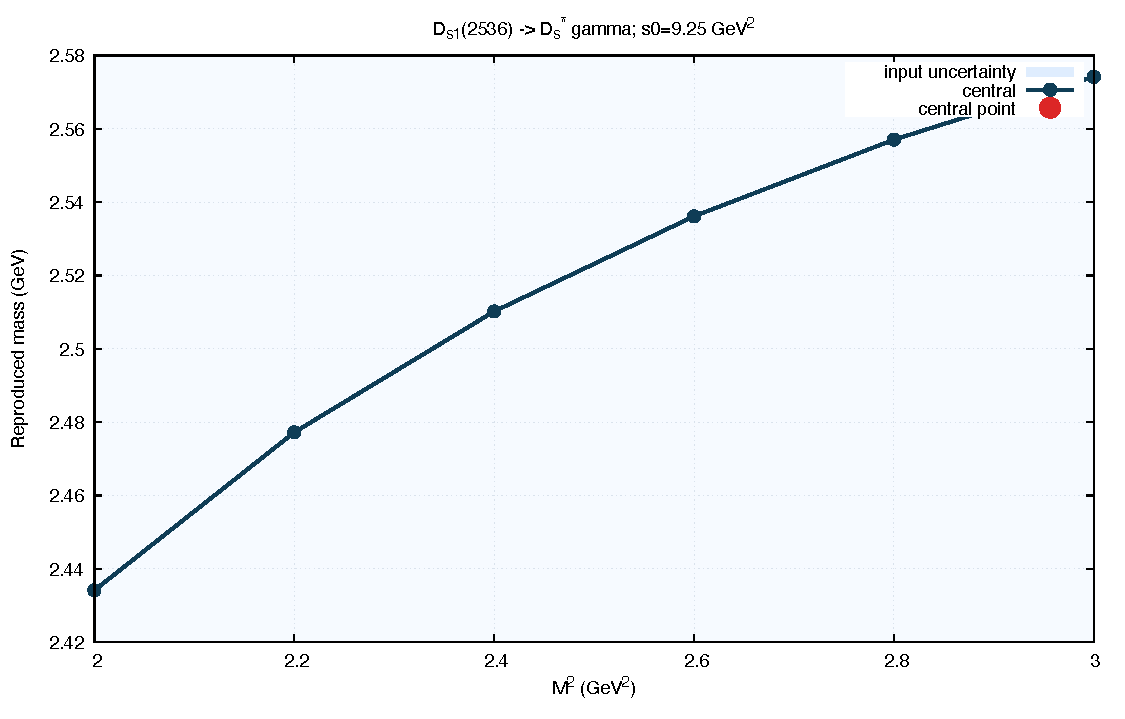
\includegraphics[width=\linewidth]{Ds1_2536_mass_sr_vs_M2.pdf}
\caption{mass reconstruction}
\end{subfigure}
\caption{Representative two-point diagnostics for $D_{s1}(2536)$.}
\end{figure}

\subsection{Comparison with previous calculations and data}

\clearpage
{\footnotesize
\setlength{\tabcolsep}{4pt}
\renewcommand{\arraystretch}{1.10}
\begin{longtable}{>{\raggedright\arraybackslash}p{0.13\linewidth}>{\raggedright\arraybackslash}p{0.23\linewidth}>{\raggedright\arraybackslash}p{0.27\linewidth}>{\raggedright\arraybackslash}p{0.28\linewidth}}
\caption{Radiative-width predictions and current experimental status.  Width entries are in keV.  ``This work'' gives the median and 16th--84th percentile interval; experimental rows report direct branching-fraction, total-width, or observation information and must not be read as radiative widths.}\label{tab:literature-full}\\
\toprule
Entry & width [keV] or experimental status & method/status & source and note\\
\midrule
\endfirsthead
\multicolumn{4}{l}{\footnotesize\itshape Table \thetable\ continued from the previous page}\\
\toprule
Entry & width [keV] or experimental status & method/status & source and note\\
\midrule
\endhead
\midrule
\multicolumn{4}{r}{\footnotesize Continued on the next page}\\
\endfoot
\bottomrule
\endlastfoot
\addlinespace[3pt]
\multicolumn{4}{l}{\textbf{$D_{s1}(2460)^+\to D_s^{\ast+}\gamma$}}\\
\textbf{This work} & \textbf{$0.482_{-0.434}^{+1.609}$} & mixed-current external-photon LCSR & this calculation\\
Published & $0.6\,\text{--}\,1.1$ & pure-axial external-photon LCSR & Colangelo et al. (2005)~\cite{Colangelo2005}; pure-A benchmark\\
Published & $1.5$ & vector-meson dominance & Colangelo et al. (2005)~\cite{Colangelo2005}\\
Published & $5.5$ & nonrelativistic quark model & Godfrey (2003)~\cite{Godfrey2003}\\
Published & $4.66$ & chiral-doublet effective theory & Bardeen et al. (2003)~\cite{Bardeen2003}\\
Published & $4.74\,\text{--}\,4.79$ & relativistic quark model & Chen et al. (2020)~\cite{Chen2020}; three parameter modes\\
Published & $15.5$ & potential-model calculation & Radford et al. (2009)~\cite{Radford2009}\\
Published & $17.4$ & potential-model calculation & Green et al. (2017)~\cite{Green2017}\\
Published & $5.6$ & relativized quark model & Godfrey (2005)~\cite{Godfrey2005}\\
Published & $4.41$ & quark model & Close and Swanson (2005)~\cite{CloseSwanson2005}\\
Published & $14.6\,\text{--}\,22.8$ & relativistic heavy-quark model & Goity and Roberts (2001)~\cite{GoityRoberts2001}; three model variants collected in Chen et al.\\
Published & $13\pm 2$ & hadronic-molecule EFT & Fu et al. (2022)~\cite{Fu2022}; full result\\
Published & $104$ & potential model with relativistic corrections & Bondar and Milstein (2025)~\cite{BondarMilstein2025}; authors estimate 50\% model uncertainty\\
\textbf{Experiment} & \textbf{$\mathcal B(D_s^\ast\gamma)<8\%$ (90\% CL); $\Gamma_{\rm tot}<3.5$ MeV} & upper limit & PDG (2026)~\cite{PDG2026}\\
\addlinespace[3pt]
\multicolumn{4}{l}{\textbf{$D_{s1}(2536)^+\to D_s^{\ast+}\gamma$}}\\
\textbf{This work} & \textbf{$0.094_{-0.089}^{+0.520}$} & mixed-current external-photon LCSR & this calculation\\
Published & $2.96\,\text{--}\,3.02$ & relativistic quark model & Chen et al. (2020)~\cite{Chen2020}; three parameter modes\\
Published & $8.90$ & potential-model calculation & Radford et al. (2009)~\cite{Radford2009}\\
Published & $9.21$ & potential-model calculation & Green et al. (2017)~\cite{Green2017}\\
Published & $0.4\pm 1.0$ & heavy-quark effective calculation & K{\"o}rner et al. (1993)~\cite{Korner1993}\\
Published & $5.5$ & relativized quark model & Godfrey (2005)~\cite{Godfrey2005}\\
Published & $1.59$ & quark model & Close and Swanson (2005)~\cite{CloseSwanson2005}\\
Published & $14.0\,\text{--}\,25.1$ & relativistic heavy-quark model & Goity and Roberts (2001)~\cite{GoityRoberts2001}; three model variants collected in Chen et al.\\
Published & $29$ & potential model with relativistic corrections & Bondar and Milstein (2025)~\cite{BondarMilstein2025}; authors estimate 50\% model uncertainty\\
\textbf{Experiment} & \textbf{mode possibly seen; no $\mathcal B$ or partial width; $\Gamma_{\rm tot}=0.92\pm0.05$ MeV} & possibly seen & PDG (2026)~\cite{PDG2026}\\
\pagebreak
\addlinespace[3pt]
\multicolumn{4}{l}{\textbf{$B_{s1}^{L\,0}\to B_s^{\ast0}\gamma$ (predicted lower state)}}\\
\textbf{This work} & \textbf{$1.589_{-1.298}^{+2.703}$} & mixed-current external-photon LCSR & this calculation\\
Published & $0.3\,\text{--}\,6.1$ & pure-axial external-photon LCSR & Wang (2008)~\cite{Wang2008}; lower strange-bottom axial partner\\
Published & $100\pm 15$ & hadronic-molecule EFT & Fu et al. (2022)~\cite{Fu2022}; lower strange-bottom molecular partner\\
Published & $60$ & nonrelativistic quark model & Li et al. (2021)~\cite{Li2021}; conditional subthreshold missing 1P1 state\\
Published & $20$ & potential model with relativistic corrections & Bondar and Milstein (2025)~\cite{BondarMilstein2025}; $B_{s1}(5748)$ assignment; authors estimate 50\% accuracy\\
\textbf{Experiment} & \textbf{state unobserved; no measurement or limit} & unobserved state & PDG (2026)~\cite{PDG2026}\\
\addlinespace[3pt]
\multicolumn{4}{l}{\textbf{$B_{s1}(5830)^0\to B_s^{\ast0}\gamma$ (observed higher state)}}\\
\textbf{This work} & \textbf{$2.332_{-1.925}^{+5.735}$} & mixed-current external-photon LCSR & this calculation\\
Published & $53$ & nonrelativistic quark model & Li et al. (2021)~\cite{Li2021}; observed higher state\\
Published & $41$ & potential model with relativistic corrections & Bondar and Milstein (2025)~\cite{BondarMilstein2025}; $B_{s1}(5829)$ assignment; authors estimate 50\% accuracy\\
\textbf{Experiment} & \textbf{radiative mode unobserved; no measurement or limit} & unobserved mode & PDG (2026)~\cite{PDG2026}\\
\end{longtable}
}


\Cref{tab:literature-full} includes our four percentile results, the
predictions in the primary comparison tables of
Refs.~\cite{Colangelo2005,Chen2020,Fu2022}, and the additional bottom-state
calculation of Ref.~\cite{Li2021}.  We also include the relativistic-potential
model of Ref.~\cite{BondarMilstein2025}, which predicts $104$ and $29$ keV for
the two charm channels and $20$ and $41$ keV for its $B_{s1}(5748)$ and
$B_{s1}(5829)$ assignments, respectively; that work estimates a 50\% model
uncertainty for these predictions.  Values quoted for several parameter modes
or model variants are compressed to their displayed range; no uncertainty
has been inferred where the source gives only a central value.  The lower
$B_{s1}^{L}$ rows of
Refs.~\cite{Wang2008,Fu2022,BondarMilstein2025,Li2021} concern predicted
near-threshold partners and are not assignments of the observed
$B_{s1}(5830)$.

Experiment does not yet provide a radiative partial width for any of the four
channels.  For $D_{s1}(2460)^+\to D_s^{\ast+}\gamma$, the direct result is the
90\% C.L.\ branching-fraction bound
$\mathcal B(D_s^\ast\gamma)<8\%$, accompanied by the independent total-width
bound $\Gamma_{\rm tot}<3.5$ MeV; these are therefore shown as limits rather
than converted into a measured width.  The $D_{s1}(2536)$ mode is listed as
possibly seen without a branching fraction, while the lower $B_{s1}^{L}$ is
unobserved and no quantitative $B_{s1}(5830)\to B_s^\ast\gamma$ limit is
available \cite{PDG2026}.

\section{Independent validation}

The symbolic Wolfram Language calculation constructs explicit Dirac matrices,
evaluates AA, AB, and BB cut traces, factorizes \cref{eq:det}, rotates the
matrix, and checks the Ward determinant.  The numerical Wolfram Language
implementation uses native adaptive integration and does not read Python
values.  Python uses Gauss--Legendre quadrature.  Their complete
42-entry comparison is machine-readable in
\path{outputs/csv/python_mathematica_regression.csv}.  All entries pass either
$2\times10^{-8}$ absolute or $2\times10^{-5}$ relative tolerance.  The
maximum material relative difference is \RegressionMaxRel; the maximum
absolute difference is \RegressionMaxAbs.

\begin{longtable}{p{0.29\linewidth}p{0.13\linewidth}p{0.50\linewidth}}
\toprule
Gate & status & evidence\\
\midrule
\endfirsthead
\toprule
Gate & status & evidence\\
\midrule
\endhead
$\rho_{AB}=\rho_{BA}$ & checked & identical function and symbolic WL equality\\
spectral positivity & checked & analytic determinant is nonnegative above threshold\\
mass dimensions & checked & rho dim 2; Borel matrix and T dim 4; g dimensionless\\
physical threshold & checked & all dispersive integrals start at (mQ+ms)\textasciicircum{}2\\
Ward identity & checked & epsilon structure vanishes under epsilon\_gamma -$>$ q\\
no local transition condensate & checked & diagnostic term excluded from quoted\_total\_A/B\\
two-point $d=3,5$ & checked & explicit matrices retained\\
pure A limit & checked & theta=90 degrees for lower state\\
pure B limit & checked & theta=0 degrees for lower state\\
equal Borel limit & checked & M1\textasciicircum{}2=M2\textasciicircum{}2=2M\textasciicircum{}2 gives u0=1/2\\
$m_s\to0$ threshold & checked & lambda and density reduce smoothly\\
charge switch & checked & hard density changes through eQ/es only\\
Python--Mathematica regression & checked & 42/42 entries pass; max material rel=9.128e-07; max abs=2.425e-06\\
subleading tensor kernels & truncation & not retained; 15\% charm and 5\% bottom correlated uncertainty assigned\\
transition $\alpha_s$ & truncation & not retained\\
\bottomrule
\end{longtable}


\section{Conclusions}

The clean-room calculation produces a fully populated two-point current
matrix, mixed-state residues, a term-resolved external-photon LCSR, four
radiative couplings and widths, stability scans, uncertainty samples, and an
independent Wolfram Language regression.  The median widths are
\DsLowWidth\ keV for $D_{s1}(2460)$, \DsHighWidth\ keV for
$D_{s1}(2536)$, \BsLowWidth\ keV for the lower $B_{s1}^{L}$, and
\BsHighWidth\ keV for $B_{s1}(5830)$, with the percentile ranges in
\cref{tab:results}.

The dominant conclusion is methodological: mixed-current interference is
numerically important, especially for the higher states, and the transition
Borel dependence prevents precision claims.  A next-order study should
derive the subleading tensor-current kernels independently for every DA,
include $\alpha_s$ corrections, revisit scale running consistently, and
calculate the second on-shell multipole.

\appendix
\section{Photon distribution amplitudes}
\label{app:das}

At $\mu=1$ GeV the two-particle shapes used in the numerical code are
\begin{align}
\phi_\gamma(u)&=6u\bar u,\\
h_\gamma(u)&=-10C_2^{1/2}(2u-1),\\
\psi^v(u)&=5[3\xi^2-1]
+{3\over64}(15\omega_\gamma^V-5\omega_\gamma^A)
[3-30\xi^2+35\xi^4],\\
\psi^a(u)&={5\over2}(1-\xi^2)(5\xi^2-1)
\left(1+{9\over16}\omega_\gamma^V
-{3\over16}\omega_\gamma^A\right),\\
{\cal A}(u)&=40u^2\bar u^2(3\kappa+1)
-24\zeta_2\bigl[u\bar u(2+13u\bar u)\nonumber\\
&\quad+2u^3(10-15u+6u^2)\ln u
+2\bar u^3(10-15\bar u+6\bar u^2)\ln\bar u\bigr],
\end{align}
where $\bar u=1-u$ and $\xi=2u-1$.

With $\alpha_q+\alpha_{\bar q}+\alpha_g=1$, the three-particle DAs are
\begin{align}
{\cal V}&=540\omega_\gamma^V
(\alpha_q-\alpha_{\bar q})\alpha_q\alpha_{\bar q}\alpha_g^2,\\
{\cal A}_3&=360\alpha_q\alpha_{\bar q}\alpha_g^2
\left[1+{\omega_\gamma^A\over2}(7\alpha_g-3)\right],\\
{\cal S}&=30\alpha_g^2\{\kappa(1-\alpha_g)
+\zeta_1(1-\alpha_g)(1-2\alpha_g)
+\zeta_2[3(\alpha_{\bar q}-\alpha_q)^2
-\alpha_g(1-\alpha_g)]\},\\
\widetilde{\cal S}&=-{\cal S},\\
{\cal T}_1={\cal T}_3&=-360\zeta_2
(\alpha_{\bar q}-\alpha_q)\alpha_q\alpha_{\bar q}\alpha_g,\\
{\cal T}_2={\cal T}_4&=30\alpha_g^2(\alpha_{\bar q}-\alpha_q)
\{\kappa+\zeta_1(1-2\alpha_g)+\zeta_2(3-4\alpha_g)\}.
\end{align}
The combinations are
\begin{equation}
{\cal F}_2={\cal S}+\widetilde{\cal S}+{\cal T}_1-{\cal T}_2
-{\cal T}_3+{\cal T}_4,\qquad
{\cal F}_3={\cal A}_3+{\cal V}.
\end{equation}
Their post-Borel integrals are
\begin{align}
I_{{\cal F}_2}&=
\int_0^{1-u_0}\!\!dv\int_0^{u_0/(1-v)}\!\!d\alpha_g\,{\cal F}_2
+\int_{1-u_0}^{1}\!\!dv\int_0^{(1-u_0)/v}\!\!d\alpha_g\,{\cal F}_2,\\
&\quad \alpha_q=u_0-(1-v)\alpha_g,\quad
\alpha_{\bar q}=1-u_0-v\alpha_g,\\
I_{{\cal F}_3}&=\int_0^{u_0}d\alpha_{\bar q}
\left[\int_{u_0-\alpha_{\bar q}}^{1-\alpha_{\bar q}}
{d\alpha_g\over\alpha_g^2}
{\cal F}_3(1-\alpha_{\bar q}-\alpha_g,\alpha_{\bar q},\alpha_g)
-{{\cal F}_3(1-u_0,\alpha_{\bar q},u_0-\alpha_{\bar q})
\over u_0-\alpha_{\bar q}}\right].
\end{align}
For the central symmetric BBK parameters at $u_0=1/2$,
$I_{{\cal F}_2}=0$ and
$I_{{\cal F}_3}=15(\omega_\gamma^A-3\omega_\gamma^V+4)/32=-285/64$.

\section{Supplementary figure index}

For every state the project contains PDF and PNG versions of $g$ and
$\Gamma$ versus $M^2$ and $s_0$, $g$ versus angle, and two-point pole
contribution, reconstructed mass, residue, and dimension-five fraction versus
$M^2$.  Each plot has a companion CSV.  This paper shows representative
panels; the detailed derivation report embeds the complete set.

\bibliographystyle{unsrt}
\bibliography{../references}
\end{document}
